\subsection{ZenHub}
ZenHub ist eine Projektmanagement-Erweiterung für GitHub.
\\
ZenHub haben wir dafür benutzt, um die Programmierung des Projektes in Hauptkategorien auf zu teilen.
Diesen Kategorien haben wir Mitarbeiter zu geteilt, sowie die eventuell benötigte Dauer, für die Erstellung der Punkte vergeben.
\\\\
ZenHub unterteilt sich in:
\begin{itemize}
	\item New Issues(Neue Hauptpunkte)
	\item Ice-Box(Eingefrorene Punkte)
	\item Backlog(Arbeitsrückstand)
	\item To Do(Muss gemacht werden)
	\item In Progress(In Bearbeitung)
	\item Done/Review(Fertig/Überprüfung) 
\end{itemize}
\begin{landscape}
	\begin{center}
		\begin{tabulary}{1\textwidth}{cc}
			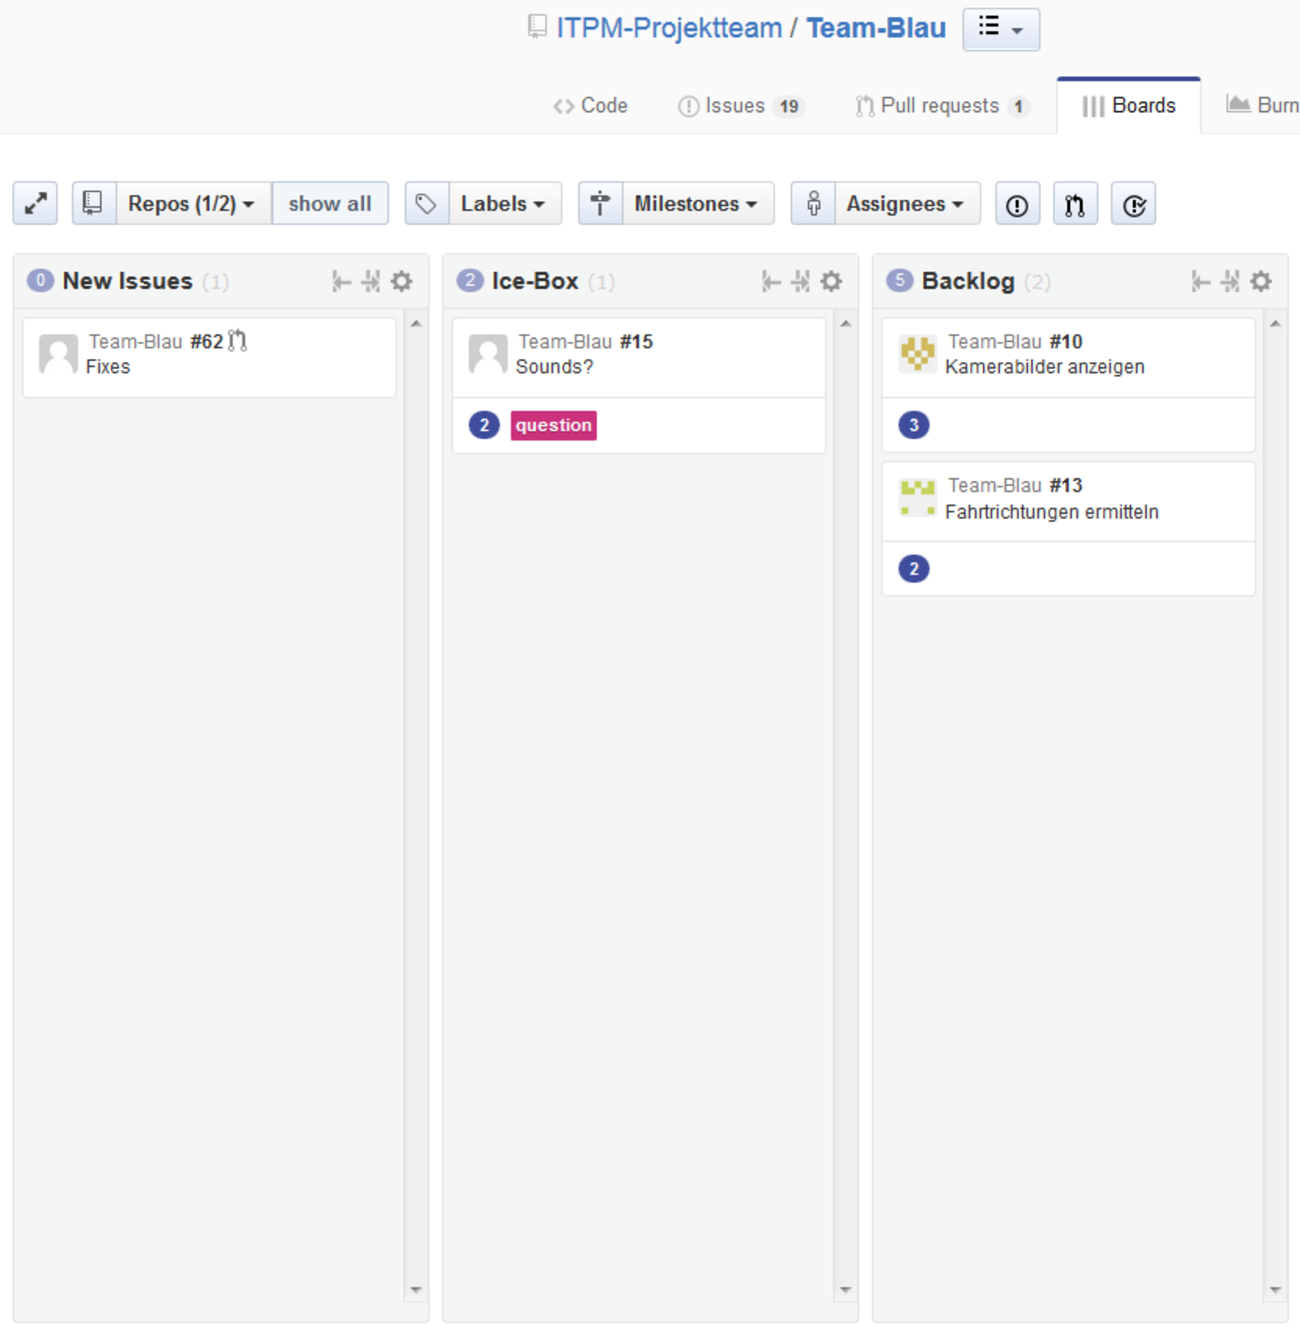
\includegraphics[scale=0.5]{Bilder/ZenHub1.pdf} 
			&
			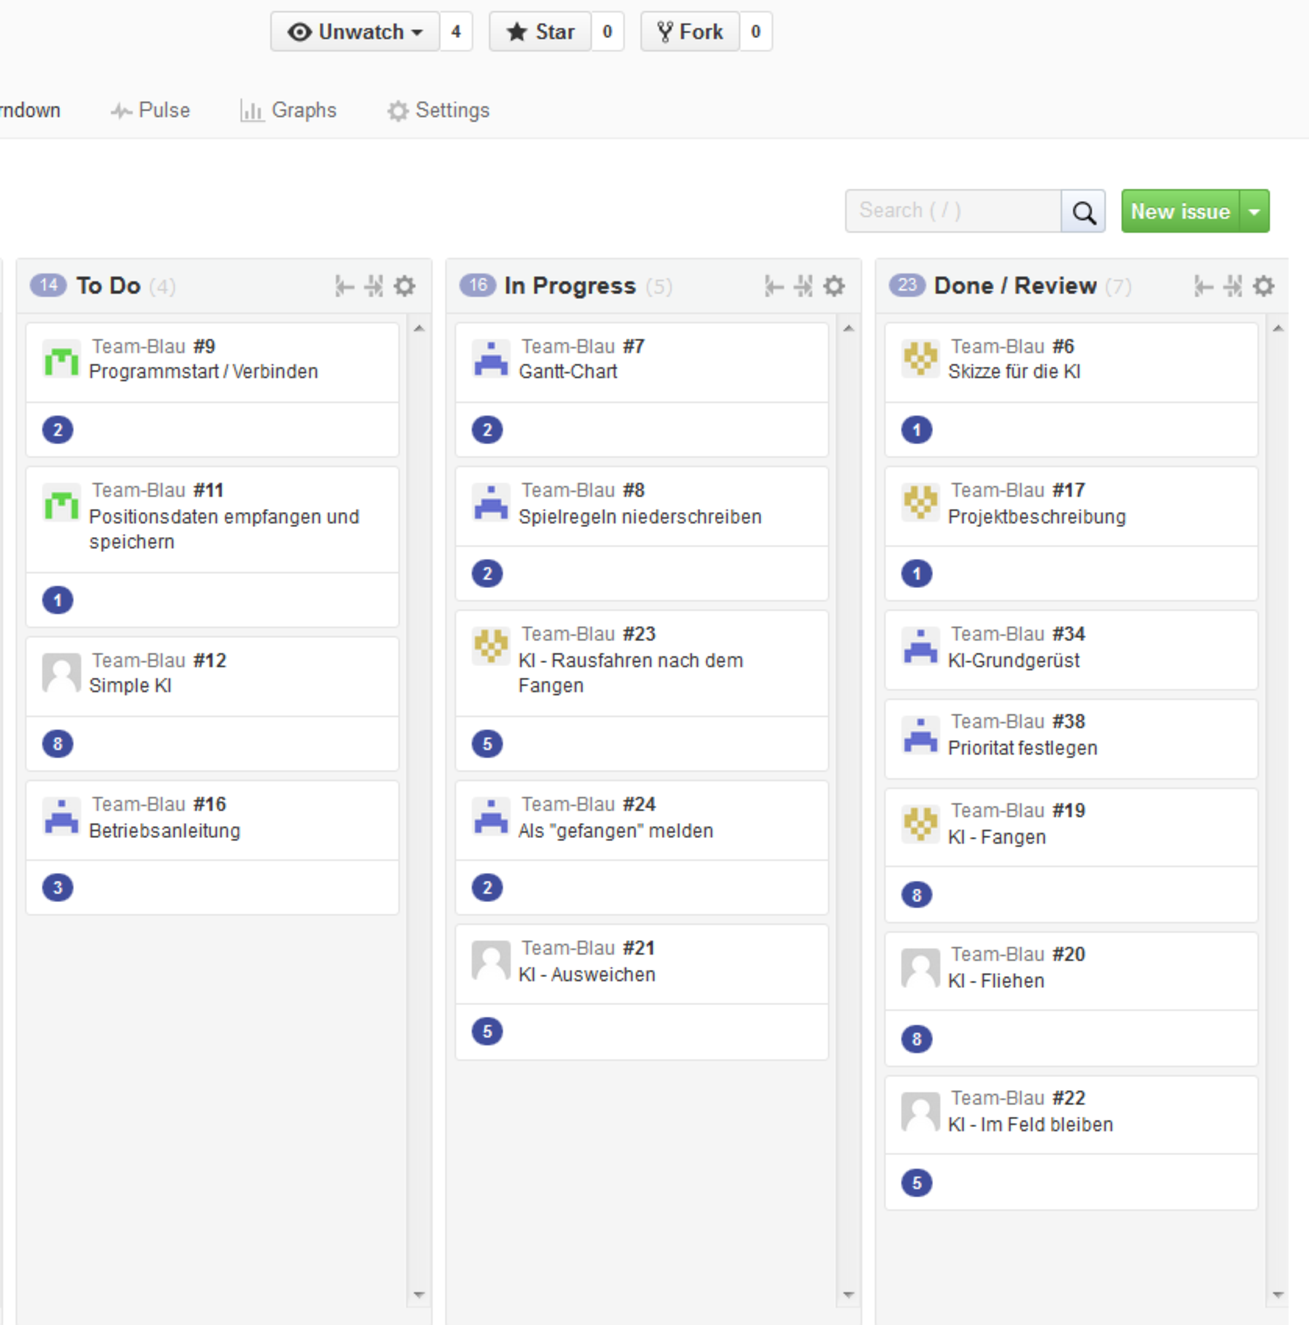
\includegraphics[scale=0.5]{Bilder/ZenHub2.pdf}\\
		\end{tabulary}
		\captionof{figure}{Auflistung der Punkte in ZenHub}
	\end{center}
\end{landscape}